\documentclass[main.tex]{subfiles}

\begin{document}




\chapter[Nuclear Chemistry]{Nuclear Chemistry}
%\label{ch:nuclear}

\begin{marginfigure}
      \includegraphics{chapter4/figure1}
   \end{marginfigure}
\lettrine[lines=4]{\color{black!45}T}{he} field of nuclear medicine was first established in 1934 with the production of artificial radioactive substances. This field uses the power of nuclear chemistry to cure cancer and other diseases or simply to visualize organs. In 1937, the first radioactive isotope was used to treat a person with leukemia at the University of California at Berkeley. Radioactive substances are now used to produce images of organs, such as liver, spleen, thyroid gland, kidneys, and the brain, and to detect heart disease. Today, procedures in nuclear medicine provide information about the function and structure of every organ in the body, which allows the nuclear physician to diagnose and treat diseases early. This chapter covers the basic principles of nuclear chemistry. You will learn the real meaning of radioactivity and how to quantify the effects of radiation or measure the duration of a radioactive chemical.
\begin{marginfigure}%LEARNING GOALS BOX
\begin{mytcbox}{GOALS}
\begin{enumerate}[label=\protect\circled{\color{white}\arabic*}]
\item Identify the different types of radiation
\item Identify the different types of nuclear decays
\item Write balanced nuclear reactions
\item Convert different activity units
\item Describe the dangers of radiation

\end{enumerate}
\end{mytcbox}
\end{marginfigure}%LEARNING GOALS BOX

\section{Radiation, particles \& radioisotopes}
Light elements have normally a stable nuclei. Differently, heavier elements with atomic numbers larger than 20 tend to often have several isotopes--remember these are atoms of the element with different number of neutrons--that have unstable nuclei. For these unstable isotopes, the forces that keep the nucleus together are not strong enough to stabilize the nuclei. A unstable nucleus are radioactive, which means that they will spontaneously emit radiation in the form of small particles. Not all radioactivity is the same and there exist different types of radiation, which we will address in the following.\sloppy 
\begin{description}
\item[\docfilehook{alpha radiation}{alpha radiation}] Alpha radiation--referred as $\alpha$--is a type of radiation that contains alpha particles. These particles are indeed helium nucleus, with 2 protons, 2 neutrons and a ($2+$) positive charge. Alpha particles are often represented as $\alpha$ or \ce{^4_2He}.
\item[\docfilehook{beta radiation}{beta radiation}] Beta radiation--referred as $\beta$--is a type of radiation that contains beta particles. These particles are indeed high-energy electrons with ($-$) negative charge. Beta particles are often represented as $\beta$ or \ce{^0_-1e}.
\item[\docfilehook{gamma radiation}{gamma radiation}] Gamma radiation--referred as $\gamma$--is a type of radiation that contains high-energy photons. These particles are indeed photons with no mass or charge. Gamma particles are often represented as $\gamma$ or \ce{^0_0\gamma}.
\end{description}
Often times in this chapter you are going to encounter several particles. You are already familiar with some of them such as electrons (\ce{^0_-1e}). In the following, we will briefly review some of the less known particles:
\begin{description}
\item[\docfilehook{protons}{protons}] Protons in this chapter are often referred as $p$ or \ce{^1_1H^+}. These are positive charges.
\item[\docfilehook{positrons}{positrons}] Positrons are the electron antiparticle, often referred as $\beta^+$ or \ce{^0_{+1}e}. They do have positive charge.
\item[\docfilehook{neutrons}{neutrons}] Neutrons are nuclear particles with no charge, often referred as $n$ or \ce{^1_{0}n}.

\item[\docfilehook{Radioisotope notation}{Radioisotope notation}] Radioisotopes--atomic isotopes that produce radiation--are named as \ce{^A_ZX}. For example, \ce{^14_6C} is referred as carbon-14. The number on to is the mass number $A$, whereas the number on the bottom is the atomic number $Z$.

  \begin{marginfigure}
\begin{tcolorbox}[enhanced,colback=red!5!white,colframe=black!50!red,boxrule=1pt,
  arc=0pt,outer arc=0pt,drop heavy lifted shadow]
\faGears\ 
\docenvdef{Discussion:} is nuclear power good or damaging for our society? List three benefits and negative consequences of nuclear power.\end{tcolorbox}
 \end{marginfigure}

\begin{example} %%%%%%%%%%%%%%%%%%%%%%%% EXAMPLE BOX
Calculate the number of protons, neutrons and electrons of the following isotopes: \ce{^238_92U }, \ce{^24_13Al} and \ce{^14_6C}.\\
\textlcsc{ \textcolor{dgreen}{\Large \textbf{Solution}} }\\
According to the isotope notation (\ce{^A_ZX}), the number of top of the radioisotope is the mass number $A$ that represents the number of protons plus neutrons, whereas the number of the bottom is the atomic number $Z$ that represents the number of electrons. According to this, the number of electrons in an atom is $Z$. If an atom is neutral, the number of electrons and protons are the same, so the number of protons is also $Z$. The number of neutrons would hence be $A-Z$, as $A$ is the number of protons+neutrons, and the number of protons is $Z$.
We'll use a table below to obtain the electrons, protons and neutrons from $A$ and $Z$.
\begin{tabularx}{\textwidth}{
    >{\centering}m{.185\linewidth} 
    *{5}{Y} }
  \toprule
\heading{Radioisotope} & \heading{$A$}  &  \heading{$Z$} & \heading{Electrons} & \heading{protons} & \heading{neutrons}   \\
    \midrule
   \ce{^238_92U } & 	238&		92&    92&		92&	146    \\
   \ce{^24_13Al} & 	24&		13&    13&		13&	11    \\
      \ce{^14_6C}& 	14&		6&    6&		6&	8\\    
    \bottomrule
\end{tabularx}
\faDiamond\ \textlcsc{ \textcolor{dgreen}{\Large \textbf{Study Check}} }\\
Calculate the number of protons, neutrons and electrons of \ce{^99_43Tc}.\\
\flushright Answer: 43e, 43p, 56n.
\end{example}%%%%%%%%%%%%%%%%%%%%%%%% EXAMPLE BOX
\end{description}
\begin{marginfigure}%%%%%%%MARGIN FIGURE
 \label{fig:prticles}
\begin{tcolorbox}[tab2,tabularx={X|Y|Y}]%%%% FANCY COLOR TABLE
Particle Name & Symbol     & Charge           \\\hline\hline
Alpha\  ($\alpha$) &    \ce{^4_2He}  & $2+$           \\\hline
Beta\  ($\beta$) &      \ce{^0_-1e}  & $-1$            \\\hline
Gamma\  ($\gamma$) &     \ce{^0_0\gamma}  & $0$           \\\hline
Proton\ ($p$) &    \ce{^1_1H^+}  & $+1$            \\\hline
Positrons\ ($\beta^+$)&     \ce{^0_{+1}e}  & $+1$            \\\hline
Neutrons\ ($n$) &   \ce{^1_{0}n}   & $0$           
\end{tcolorbox}%%%% FANCY COLOR TABLE
 \end{marginfigure}%%%%%%%MARGIN FIGURE

\section{Nuclear reactions}
Isotopes--called emitters--spontaneously decompose producing a new isotopes in a process called radioactive decay. In this decay, radiation is also emitted. 
\[ \text{Emitter} \longrightarrow \text{radiation} + \text{New isotope} \]
In the following, we will discuss the most important type of radioactive decay.
\sloppy 
\begin{description}
\item[\docfilehook{alpha decay}{alpha decay}] Some isotopes produce alpha radiation, that is, they produce $\alpha$ particles on its decay. A nuclear reaction that produces an $\alpha$ particle (\ce{^4_2He}) is called alpha decay. In an alpha decay, the emitter decreases its mass number $A$ four units and its atomic number $Z$ two units.
\[ \text{Emitter} \longrightarrow \text{\ce{^4_2He}} + \text{New isotope} \]

\item[\docfilehook{beta decay}{beta decay}] Other isotopes produce beta radiation, that is, they produce $\beta$ particles on its decay. A nuclear reaction that produces a $\beta$ particle (\ce{^0_-1e}) is called beta decay. In a beta decay, the emitter has the same mass number $A$ as the product isotope. However, its atomic number $Z$ decreases one unit.
\[ \text{Emitter} \longrightarrow \text{\ce{^0_-1e}} + \text{New isotope} \]

\item[\docfilehook{positron emission}{positron emission}] Certain isotopes decay by producing a positron, that is, they produce  \ce{^0_{+1}e}  particles on its decay. A nuclear reaction that produces \ce{^0_{+1}e} is called positron emission. In a positron emission, the emitter has the same mass number $A$ as the product isotope. However, its atomic number $Z$ increases one unit.
\[ \text{Emitter} \longrightarrow \text{ \ce{^0_{+1}e}} + \text{New isotope} \]
\item[\docfilehook{gamma decay}{gamma decay}] Some other isotopes produce gamma radiation, that is, they produce $\gamma$ particles on its decay. A nuclear reaction that produces a $\gamma$ particle (\ce{^0_0\gamma}) is called gamma decay and in this type of decay no new isotope is produced. The emitter that is normally excited--we denote this with a $^\ast$ symbol--just looses energy and becomes more stable. In a gamma decay, the emitter and the product isotope, both have the same mass and atomic number.
\[ \text{Emitter} \longrightarrow \text{\ce{^0_0\gamma}} + \text{New isotope} \]

\begin{marginfigure}%%%%%%%QUOTES
    \begin{shadequote}[l]{Einstein}
Nuclear power is one hell of a way to boil water.
\end{shadequote}   \end{marginfigure}%%%%%%QUOTES

\begin{example} %%%%%%%%%%%%%%%%%%%%%%%% EXAMPLE BOX
Label the following nuclear reactions as: $\alpha$, $\beta$ or $\gamma$ decay, or positron emission:
\begin{multicols}{2}
\begin{enumerate}[label=(\alph*)]
\item \ce{^238_92U -> ^234_90Th + ^4_2He}
\item \ce{^24_13Al -> ^24_12Mg + ^0_{+1}e}
\item \ce{^14_6C -> ^14_7N + ^0_{-1}e}
\item \ce{^99_43Tc^* -> ^99_43Tc + ^0_{0}\gamma}
\end{enumerate}
\end{multicols}
\textlcsc{ \textcolor{dgreen}{\Large \textbf{Solution}} }\\
(a) This process produces \ce{^4_2He} and therefore is alpha emission. (b) This process generates \ce{^0_{+1}e} and therefore is positron emission. (c) This process produces \ce{^0_{-1}e} and therefore is beta emission. (d) This process produces \ce{^0_{0}\gamma} and therefore is gamma emission.  \\
\faDiamond\ \textlcsc{ \textcolor{dgreen}{\Large \textbf{Study Check}} }\\
Label the following nuclear reactions as: $\alpha$, $\beta$ or $\gamma$ decay, or positron emission:
\begin{multicols}{2}
\begin{enumerate}[label=(\alph*)]
\item \ce{^127_55Cs -> ^127_54Xe + ^0_{+1}e}
\item \ce{^27_13Al^* -> ^27_13Al + ^0_{0}\gamma}
\item \ce{^218_85At -> ^214_83Bi + ^4_{2}He}
\end{enumerate}\end{multicols}
\flushright Answer: (a) positron emission; (b) gamma emission; (c) alpha emission.
\end{example}%%%%%%%%%%%%%%%%%%%%%%%% EXAMPLE BOX
\end{description}

\section{Unknown isotopes in nuclear reactions}
Sometimes one needs to identify an unknown isotope \ce{^A_ZX} in a chemical reaction. This means identify the name $X$ of the isotope, the atomic number $Z$ as well as the mass number $A$. In order to do this, we will use the fact that the total mass number as well as the total atomic number should stay constant before and after the nuclear reaction. Let's break this idea down in an example.
\begin{example} %%%%%%%%%%%%%%%%%%%%%%%% EXAMPLE BOX
Identify the unknown isotope in the following nuclear reaction:\\
\centerline{ \ce{^4_2He + ^14_7N -> ^A_ZX + ^1_{1}H}}\\
\textlcsc{ \textcolor{dgreen}{\Large \textbf{Solution}} }\\
We will solve this problem by using the fact that the total mass number as well as the total atomic number should stay constant before and after the nuclear reaction. In order to do this, we will calculate the total atomic number before the reaction (in the left) and the total atomic number after the reaction (in the right) and equal both values. We will do the same for the mass number.
\begin{tabularx}{\textwidth}{
    >{\centering}m{.185\linewidth} 
    *{5}{Y} }
  \toprule
&\heading{\ce{^4_2He}} & \heading{\ce{^14_7N}}  &  \heading{\ce{->}} & \heading{\ce{^A_ZX}} & \heading{\ce{^1_1H}}   \\
    \midrule
  A  &4 &14    &    &$A$  &1    \\
    \midrule 
    Z  &2 &7    &    &$Z$  &1    \\
    \bottomrule
\end{tabularx}
Now we build up two equations, one for $A$ and another for  $Z$, from each of the columns (column 2 and 3) of the table:
\begin{align}
 4 +14  =A  +1                  \tag*{Equation for A from column 2 of the table}
  \\2 +7  =Z  +1                  \tag*{Equation for Z from column 3 of the table}
\end{align}
We now solve for $A$ geting a value of $A=17$ and for $Z$, getting $Z=8$. With the atomic number $Z$ we can go to the periodic table and identify the name of the isotope. The element with $Z=8$ is called oxygen, and the final answer would be: \ce{^17_8O}.\\
\faDiamond\ \textlcsc{ \textcolor{dgreen}{\Large \textbf{Study Check}} }\\
Identify the unknown isotope in the following nuclear reaction:\\
\centerline{ \ce{^241_95Am -> ^A_ZX + ^4_{2}He}}
\flushright Answer: \ce{^237_93Np}
\end{example}%%%%%%%%%%%%%%%%%%%%%%%% EXAMPLE BOX

\begin{marginfigure}[7cm]
\begin{tcolorbox}[tab2,tabularx={XY}]%%%% FANCY COLOR TABLE
\begin{center}Radioisotope \end{center} & \begin{center}$t_{1/2}$  \end{center}        \\\hline\hline
\ce{^14_16C} & 5730 y          \\\hline
\ce{^40_19K} & $1.3\times 10^9$ y          \\\hline
\ce{^226_88Ra} & 1600 y          \\\hline
\ce{^90_38Sr} & 38 y          
\end{tcolorbox}%%%% FANCY COLOR TABLE
\caption{Table with half-lives for several isotopes}
\label{tab:halflife}
\end{marginfigure}

\section{Half-life of a radioisotope}
Radioisotopes--isotopes that decay producing radiation-- are unstable and with time they eventually disappear given a more stable isotope. Some radioisotopes decay very quickly, such as the one used in nuclear medicine to fight cancer. Other radioisotopes take longer to disappear. The half-life of an isotope $t_{1/2}$ is the time it takes for an isotope to disappear reducing the sample mass to half the initial value. For example, $t_{1/2}$ for chromium-51is 28 days and that means that after that time a one gram sample of the radioisotope will weight 0.5 g. $t_{1/2}$ for strontium-90 is 38 years that means that a one gram sample will take 38 years to reduce its mass to 0.5g. The formula that related the amount of radioisotope with $t_{1/2}$ is:
\resizeableyellownote{2.5}{1}{Add Equation \ref{formula4:1} to your flashcard.}
\begin{equation} \boxed{    N(t)=N_o\cdot 0.5^{\big(\dfrac{t}{t_{1/2}}\big)}  } \label{formula4:1}\end{equation}
where $N(t)$ is the amount of isotope at a given time $t$, $N_o$ is the initial amount of isotope, $t$ is the time and $t_{1/2}$  is the half-life. $N(t)$ is often referred as the activity of the radioisotope at a give time $t$. At the same time, while the radioisotope disappear, a new isotope--this time more stable than the radioisotope--starts forming. The amount of product formed $F(t)$ at a given time is:
\resizeableyellownote{2.5}{1}{Add Equation \ref{formula4:2} to your flashcard.}
\begin{equation} \boxed{    F(t)=N_o\cdot \Big[1-0.5 ^{\big(\dfrac{t}{t_{1/2}}\big)} \Big] } \label{formula4:2}\end{equation}
\begin{description}
\item[\docfilehook{after several half-lives}{after several half-lives}] So if half-life is the time it takes for a radioisotope to decompose in half, what would happen after several half-lives? For example, imagine we have 20 grams of iridium-131 with a half-life of 8 days. When we prepare or hypothetically unseal the sample, we will have 20 grams of \ce{^131 Ir}. After one half-life (8 days) we'll have 10 grams of \ce{^131 Ir}. After two half-lives (16 days), we'll have 5 grams of \ce{^131 Ir}. Similarly, after three half-lives (22 days), we'll have 2.5 grams.
\end{description}
\begin{marginfigure}[0cm]%%%%%%%MARGIN PLOT
\begin{tikzpicture}[yscale=0.8]
\begin{axis}[axis background/.style = {%
      shade,
      top color = blue!10,
      bottom color = white},
    x tick label style={
        /pgf/number format/1000 sep=},
    ymax=19,%
    ymin=1,%
    title={ \boxed{\ce{^131_53Ir -> ^131_54Xe + ^0_{-1}e}} },
    xmax=40,%
    xmin=0,%
    width=\linewidth,
    enlargelimits=0.1,
    legend style={at={(0.5,0.5)},
      anchor=north,legend columns=-1},
    ylabel={\Large $N(t)$ of \ce{^131_53Ir} (g)},xlabel={\Large Time (days)},
    bar width=5mm, y=4mm,
    symbolic x coords={0, 8, 24, 32, 40},
    xtick=data,
    nodes near coords align={vertical},
    ]
\addplot[ybar,  fill=black!10] 
    coordinates {(0,20) (8,5) (24,2.5) (32,1.25) (40,0.6)} ;
    \node [above] at (axis cs:  8,5) {$t_{1/2}$};
        \node [above] at (axis cs:  24,2.5) {$2t_{1/2}$};
        \node [above] at (axis cs:  32,1.25) {$3t_{1/2}$}; 
\end{axis}
    \end{tikzpicture}
    \begin{tikzpicture}[yscale=0.8]
\begin{axis}[axis background/.style = {%
      shade,
      top color = red!10,
      bottom color = white},
    x tick label style={
        /pgf/number format/1000 sep=},
    ymax=19,%
    ymin=1,%
    xmax=40,%
    xmin=0,%
    width=\linewidth,
    enlargelimits=0.1,
    legend style={at={(0.5,0.5)},
      anchor=north,legend columns=-1},
    ylabel={\Large $N(t)$ of \ce{^131_54Xe} (g)},xlabel={\Large Time (days)},
    bar width=5mm, y=4mm,
    symbolic x coords={0, 8, 24, 32, 40},
    xtick=data,
    nodes near coords align={vertical},
    ]
\addplot[ybar,  fill=black!10] 
    coordinates {(0,0) (8,15) (24,17) (32,18) (40,19)} ;
    \node [above] at (axis cs:  8,15) {$t_{1/2}$};
        \node [above] at (axis cs:  24,17) {$2t_{1/2}$};
        \node [above] at (axis cs:  32,18) {$3t_{1/2}$};  
      
\end{axis}
    \end{tikzpicture}
\end{marginfigure}%%%%%%%MARGIN PLOT



\begin{example} %%%%%%%%%%%%%%%%%%%%%%%% EXAMPLE BOX
\ce{^131_53I} has a half-life of 8days. How many milligrams of a 50mg sample will remain after 10 days.
\\
\textlcsc{ \textcolor{dgreen}{\Large \textbf{Solution}} }\\
We will following steps to solve this problem:
\begin{enumerate}[label=\protect\circled{\color{white}\arabic*}]
\item \begin{bf}Step one:\end{bf} list of the given variables.
%%% DATA BOX
\begin{tcbitemize}[raster columns=3, raster rows=3, enhanced, sharp corners, raster equal height=rows, raster force size=false, raster column skip=0pt, raster row skip = 0pt]
%Empty corner and two headers
\tcbitem[blankest, width=1cm]
\tcbitem[header = helpful]
\texta
\tcbitem[header = harmful]
\textb
%First row
\tcbitem[firstcol = internal]
\textcn
\tcbitem[swotbox = G]
$t_{1/2}=8\text{days}$ \\
$N_o=50mg$ \\
$t=10days$ \\
\tcbitem[swotbox = A]
$N(t)$
\end{tcbitemize}%%% DATA BOX
\item \begin{bf}Step two:\end{bf} use the half-life formula $N(t)=N_o\cdot 0.5^{\dfrac{t}{t_{1/2}}}  $ to obtain the mass remaining of the radioisotope\vspace*{0.1\baselineskip}
 %%%% COMMENTED EQUATION
\vspace{15mm}\begin{equation*}
N(t)=\,\,\,\,\tikzmark{A}{$N_0$}\,\,\,\,\cdot 0.5\,\,^{\dfrac{  \,\,\,\,\tikzmark{L}{t}\hspace{1em} }{  \tikzmark{G}{\,\,\,$t_{1/2}$}  }}
\end{equation*}
\begin{tikzpicture}[overlay, remember picture,node distance =1.5cm]
    \node (Adescr) [below left=of A ]{50mg};
    \draw[,->,thick] (Adescr) to [in=-90,out=90] (A);
    \node[red] (Gdescr) [below =of G]{8d};
    \draw[red,->,thick] (Gdescr) to [in=-90,out=90] (G);
   \node[blue,xshift=1cm] (Ldescr) [above right =of L]{10d};
    \draw[blue,->,thick] (Ldescr) to [in=45,out=-90] (L.north);

    \end{tikzpicture}\vspace{12mm} %%%% COMMENTED EQUATION
\item \begin{bf}Step three:\end{bf} solve for $N=50 \cdot 0.5^{\dfrac{10}{8}}=50 \cdot 0.5^{1.25}=21mg$. The result means that after 10 days from the 50mg sample of radioisotope, only 21mg will remain due to radioactive decay.
\end{enumerate}
\faDiamond\ \textlcsc{ \textcolor{dgreen}{\Large \textbf{Study Check}} }\
\ce{^222_86Rn} has a half-life of 3.8 days. How many milligrams of a 25mg sample will remain after 15 days.\\
\flushright Answer: 1.6mg.
\end{example}%%%%%%%%%%%%%%%%%%%%%%%% EXAMPLE BOX
\marginnote[-4cm]{\faBicycle\ Remember: to solve this you need to type in the calculator:  50\keystroke{x}$0.5$\keystroke{$\wedge$}1.25.}        



\section{Radiation measurement, units and radiation effects}
Beta and gamma radiation can be detected with a  Geiger counter, which consists of a detector tube with a specific ionizing gas. When radiation enters the Geiger counter, it generates charged particles that produce a detectable electrical current. The larger the current the stronger the radioactive source. In the following we will address the different units of radioactivity--activity, adsorbed dose and biological damage--as well as the effects of radiation.
\begin{marginfigure}[-4cm]%%%%%%%MARGIN FIGURE
      \includegraphics{chapter4/figure2}
      \label{fig:marginfig}
      \caption{An old Geiger counter used to measure radiation}
	\end{marginfigure}%%%%%%%MARGIN FIGURE

\begin{description}
\item[\docfilehook{Activity units}{Activity units}] The radioactivity of an isotope, often referred as \emph{activity}, can be measure in two different units: Curies (Ci) or becquerel (Bq). Curie was somehow the original unit employed to measure the radioactivity of radium and becquerel is a more modern unit of radioactivity. Bq is the SI unit of activity. Both units are related by:
\resizeableyellownote{2.5}{1}{Add Equations \ref{formula4:3} to your flashcard.}
\begin{equation}\boxed{    1 Ci=3.7 \times10^{10} Bq   } \hspace{0.5cm} \text{or} \hspace{0.5cm}   \boxed{\frac{1 Ci}{3.7 \times10^{10} Bq}}\hspace{0.5cm} \text{or} \hspace{0.5cm}   \boxed{\frac{3.7 \times10^{10} Bq}{1 Ci}} \label{formula4:3}\end{equation}
Activity refers to the isotope and is also measured in disintegration per minute (cpm).
\item[\docfilehook{Adsorbed dose}{Adsorbed dose}] Whereas activity refers to the isotope, the adsorbed dose refers to the body that receives radiations. The unit for adsorbed dose is call rad (radiation adsorbed dose).This unit refers to the amount of radiation adsorbed per gram of material. The SI unit for adsorbed dose is the gray (Gy).

\item[\docfilehook{Radiation equivalent in humans, rem}{Radiation equivalent in humans, rem}] Not all radiations have the same impact on the human body. The radiation equivalent in humans takes into account the different types of radiation in order to adjust the biological damage of radiations. the rem is the number of rads times a factor that depends on the radiation. This factor is one for beta and gamma radiation, being 20 for alpha particles.




\item[\docfilehook{Exposure to radiation}{Exposure to radiation}] 
We are all somehow exposed to radiation every day. The reason for this background radiation is that there are many natural radioisotopes that form the atoms of many materials such as brick, concrete, water or even the air. Still, the daily exposure is very low and you should not be concern by the effect of this background radiation. 


\begin{marginfigure}[-11cm]%%%%%%%MARGIN FIGURE
      \includegraphics[width=1\textwidth]{chapter4/figure5}
      \caption{Nurses expose to radiation wear film badges to detect radiation exposure}
	\end{marginfigure}%%%%%%%MARGIN FIGURE
	
\begin{marginfigure}[-3cm]
\begin{tcolorbox}[tab2,tabularx={>{\bfseries\centering\hsize=0.1\hsize}X|>{\hsize=0.95\hsize}X},title=\Large{Radiation Measurement},boxrule=0.5pt]%%%% FANCY COLOR TABLE
\multirow{4}{*}{ \rotatebox[origin=c]{90}{ \begin{bf}Activity\end{bf}} }
&curie (Ci) \vspace{0.1cm}     \\ \cline{2-2}   
&Becquerel (Bq) = $\text{2.7}\times 10^{-11}$ Ci \vspace{0.1cm}          \\ \cline{2-2} 
&1Ci = $2.22\times10^{12}$  dpm \vspace{0.1cm}     \\\hline
\multirow{3}{*}{ \rotatebox[origin=c]{90}{ \begin{bf}Dosage (D)\end{bf}} }
&rad  \vspace{0.6cm}       \\ \cline{2-2} 
&gray (Gy) =100rad  \vspace{0.6cm}        \\\hline 
\multirow{3}{*}{ \rotatebox[origin=c]{90}{ \begin{bf}Damage (H)\end{bf}} }
&rem    \vspace{0.6cm}      \\ \cline{2-2} 
&Sievert (Sv) = 100rem \vspace{0.6cm}         \\\hline
\multicolumn{2}{c}{\begin{bf}rem=rad $\times$ Factor\end{bf}}\vspace{0.4cm} \\\hline
\end{tcolorbox}%%%% FANCY COLOR TABLE
\label{tab:protect}
\end{marginfigure}
\item[\docfilehook{Dangers of radiation}{Dangers of radiation}] 
Radiation units different than Ci or Bq are used to measure the impact of radiation in humans. The rem (radiation equivalent in humans) is a radiation unit that measures the direct biological effects of different kinds of radiation. The amount of rems a person receives would determine the impact of the radiation on this person\textquotesingle s health. As an example, radiation exposure under 25 rem are harmless and they cannot be detected. If a victim is exposured to 100 rem or higher, the person will suffer the symptoms of radiation sickness, and will feel nausea, vomit, fatigue, and a reduction in white-cell count. If a person is exposed to a dosage greater than 300 rem, that can lower the white-cell count to zero; the victim will suffer diarrhea, hair loss, and infection. Exposure to radiation of about 500 rem is expected to cause death in half of the people receiving that dose. Radiation dosages of about 600 rem would be fatal to all humans within a few weeks.


\begin{example} %%%%%%%%%%%%%%%%%%%%%%%% EXAMPLE BOX
\begin{wrapfigure}{l}{0.07\textwidth}
    \centering
    \includegraphics[width=0.1\textwidth]{./chapter4/figure3}
\end{wrapfigure}
Ioflupane is a radiopharmaceutical that helps visualize the brain of Parkinson patients. A injection of this drug has a 5mCi activity. Convert this value to MBq.
\\
\textlcsc{ \textcolor{dgreen}{\Large \textbf{Solution}} }\\
You need to use the conversion factor between Bq and Ci, $ \frac{1 Ci}{3.7 \times10^{10} Bq} $, as well as the conversion factor between mCi and Ci $ \frac{1 mCi}{1 \times10^{-3} Ci} $, and Bq and MBq $ \frac{1 MBq}{1 \times10^{6} Bq} $.
 \begin{equation*}
5\cancel{mCi} \times \dfrac{1 \times10^{-3}\cancel{Ci}}{1\cancel{mCi}} \times \dfrac{3.7 \times10^{10}\cancel{Bq}}{1\cancel{Ci}}  \times \dfrac{1MBq}{1 \times10^{6}\cancel{Bq}}  =185 MBq
\end{equation*}


\faDiamond\ \textlcsc{ \textcolor{dgreen}{\Large \textbf{Study Check}} }\\

Quadramet is a radiopharmaceutical used treat pain when cancer has spread to the bone. A injection of this drug has a 740 MBq activity. Convert this value to mCi.
\begin{wrapfigure}{l}{0.03\textwidth}
    \centering\includegraphics[width=0.07\textwidth]{./chapter4/figure4}
\end{wrapfigure} \\
\flushright Answer: $20mCi$.
\end{example}%%%%%%%%%%%%%%%%%%%%%%%% EXAMPLE BOX
\marginnote[-5cm]{\faBicycle\ Remember: the number $1 \times10^{6}$ should be typed in a calculator as:  1\keystroke{EE}$6$}        
\end{description}



\section{Radiation protection}
Radioactivity results from the emission of very energetic and small particles. It can be extremely harmful when no proper protection is used. Therefore, all hospital personnel working with radioactive isotopes--radiologist, doctor, and nurse--need to be protected against radiation. 
\sloppy 
\begin{description}
\item[\docfilehook{alpha particles}{alpha particles}] Alpha radiation is made of very heavy particles (He nuclei) that can only travel between 2-4cm in the air before disappearing Inside your body they can penetrate only 0.05mm. A simple piece of thin clothing, a lab coat, gloves or even our skin can protect us against alpha particles. 
\item[\docfilehook{beta particles}{beta particles}] Beta radiation is made of lighter particles (electrons) that move much faster than alpha particles. Beta particles travel between 200-300cm in the air and between 4-5mm in body tissue. Heavy clothing such as lab coats or gloves is needed to protect you against this radiation.
\item[\docfilehook{gamma particles}{gamma particles}] Gamma radiation can pass through many materials such including body tissues. Gamma rays travel around 500 m in the air, and more than 50cm in tissue. Only very dense shielding, such as lead or concrete, will protect you from this radiation. 


\begin{marginfigure}[-8cm]
\begin{tcolorbox}[tab2,tabularx={>{\bfseries\centering\hsize=0.1\hsize}X|>{\hsize=0.90\hsize}X},title=\Large{Radiation Protection},boxrule=0.5pt]%%%% FANCY COLOR TABLE
\multirow{4}{*}{ \rotatebox[origin=c]{90}{ \begin{bf}$\alpha$ particle\end{bf}} }
&Travels 2-4cm in air \vspace{0.1cm}     \\ \cline{2-2}   
&Travels 0.05mm in tissue \vspace{0.1cm}          \\ \cline{2-2} 
&protected with thin clothing  \vspace{0.1cm}     \\\hline
\multirow{4}{*}{ \rotatebox[origin=c]{90}{ \begin{bf}$\beta$ particle\end{bf}} }
&Travels 200-300cm in air   \vspace{0.1cm}       \\ \cline{2-2} 
&Travels 4-5mm in tissue  \vspace{0.1cm}       \\ \cline{2-2} 
&protected with heavy clothing  \vspace{0.1cm}     \\\hline
\multirow{4}{*}{ \rotatebox[origin=c]{90}{ \begin{bf}$\gamma$ particle\end{bf}} }
&Travels 500m in air    \vspace{0.1cm}      \\ \cline{2-2} 
&Travels 50cm in tissue \vspace{0.1cm}        \\ \cline{2-2} 
&protected with lead or concrete \vspace{0.1cm}   \\\hline
\end{tcolorbox}%%%% FANCY COLOR TABLE
\label{tab:protect}
\end{marginfigure}
\end{description}

\section{Radioactive gases: radon}
Radon is a colorless, odorless radioactive gas produced by the radioactive decay of uranium. It is present in nearly all soils and very small levels of radon are found in the air we breathe every day. The problem occurs when radon gas enters our home and gets trapped. If you are breathing in too much radon, you will not feel sick right away. Only long-term exposure to high levels of radon can cause lung cancer and the risk is higher for those who smoke. While questions still remain over the quantities and length of exposure, radon concerns are a fact of homeownership. Most residential real estate transactions require radon testing, and many states require radon mitigation for new construction. The recommended reference radon level is 100 $Bq\cdot m^3$ in dwellings. 
Testing your home for radon is easy and doesn't cost very much. You can test for radon yourself or hire a professional to do it for you. There are relatively simple tests for radon gas. Radon detection devices are commercially available. Digital radon detectors provide ongoing measurements giving both daily, weekly, short-term and long-term average readouts via a digital display. Short-term radon test devices used for initial screening purposes are inexpensive, in some cases free.

\section{Fusion and fission}
This section will address nuclear fusion and fission. These two processes involve the liberation of a very large amount of energy and are the base for using nuclear processes as a source of energy.
\begin{marginfigure}[-11cm]%%%%%%%MARGIN FIGURE
      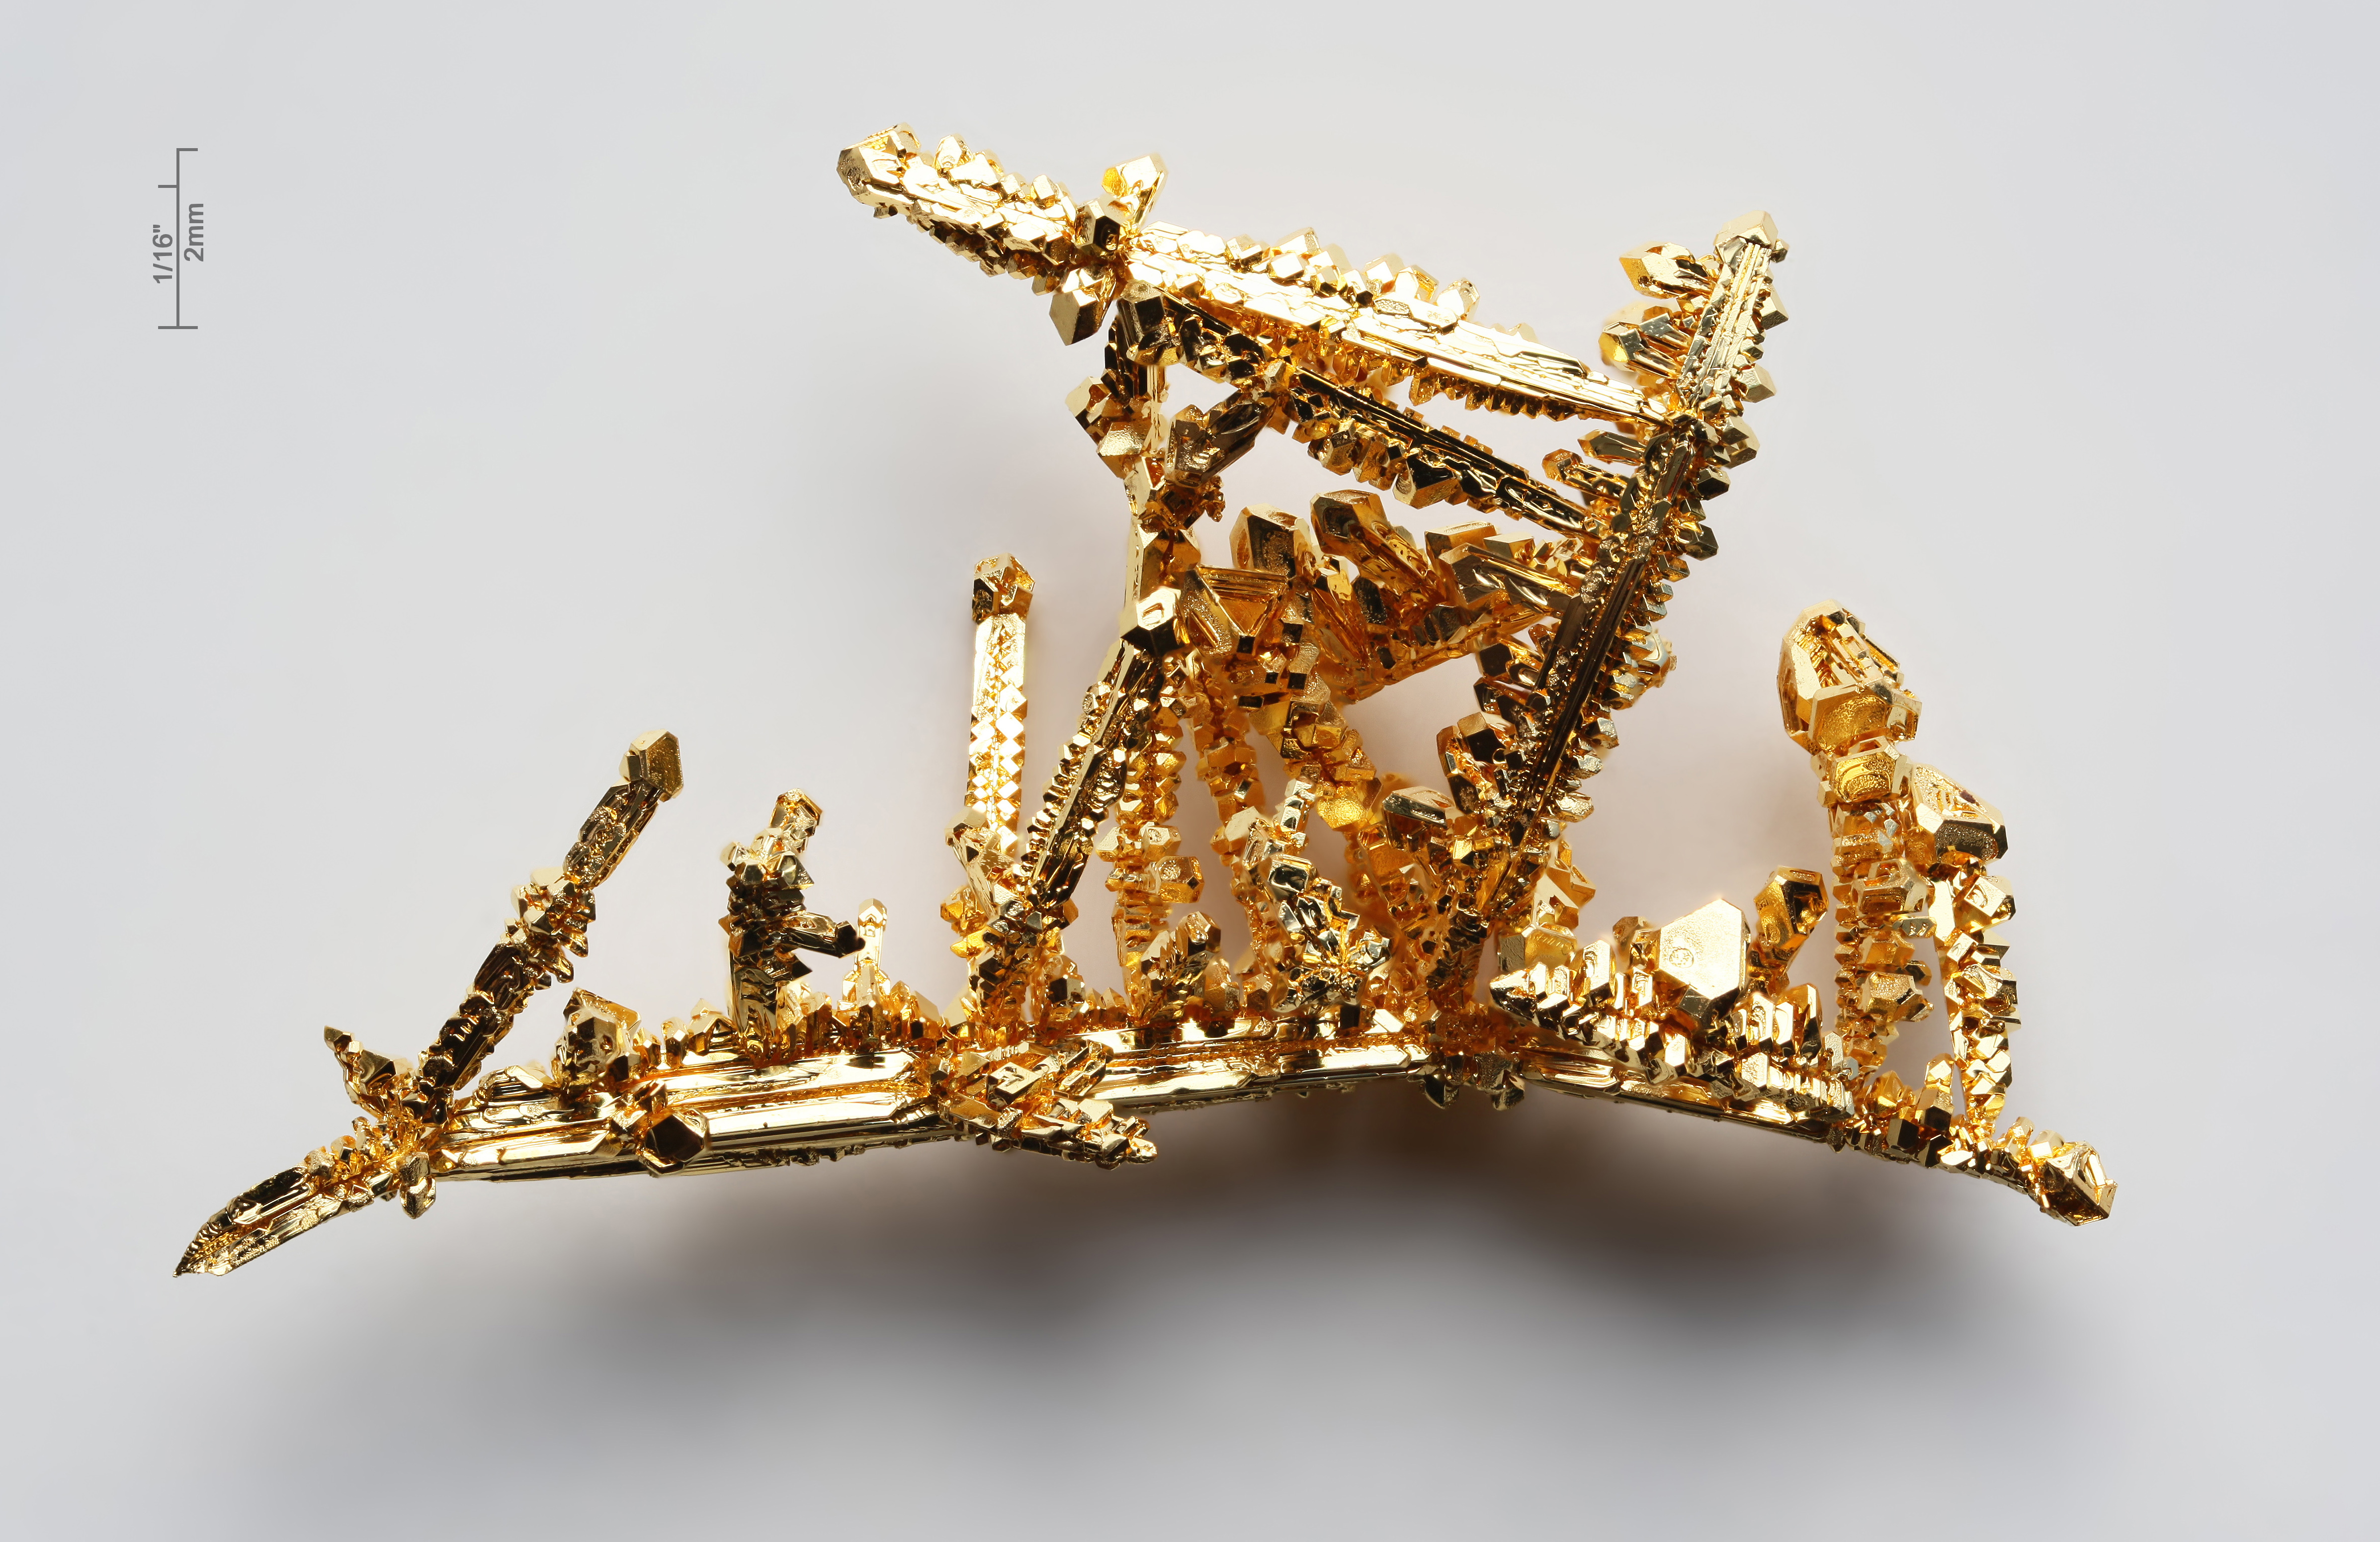
\includegraphics[width=0.9\textwidth]{chapter4/figure6}
      \caption{Nuclear weapons are based on the principles of fission.}
	\end{marginfigure}%%%%%%%MARGIN FIGURE
\sloppy 
\begin{description}
\item[\docfilehook{Nuclear fusion}{}] Large energy quantities are releases when two light isotopes combine to produce a heavier isotope. Nuclear fusion is the mechanism of energy production in the stars. Very high temperatures are required to initiate nuclear fusion and that is the reason why this source of energy has not been exploited in the earth yet. An example of fusion reactions found in the stars are:
\begin{center}\ce{^1_1H + ^2_1H -> ^3_2He }\\
\ce{^3_2He + ^1_1H -> ^4_2He + ^0_1e }
\end{center}
\item[\docfilehook{Nuclear fission}{}] Nuclear fission was discovered in before the second world war when \ce{^235_92U} was bombarded with neutrons. The result is the split of the atom in two different isotopes and the release of more neutrons:
\begin{center}\ce{^1_0n + ^235_92U -> ^141_56Ba + ^92_36Kr + 3^1_0n }\end{center}
This process releases 26 million times more energy than the combustion of methane. As neutrons are produced in a fission process, they can already activate another uranium atom producing more neutrons. This is the essence of a chain reaction: a self-sustained fission process. If less than one neutron causes a new fission process the fission process will stop and the reaction is said to be subcritical. Differently, when exactly one neutron from each fission even produces another fission the process will sustain and the reaction is know as critical. When more than one neutron produced generates a new fission the fission process will escalate and the reaction is known as supercritical. During the World War II, the Manhattan project was a united states research project with the aim to build a bomb based on the principles of fission. A fission bomb operates by suddenly combining subcritical masses of uranium, producing a enormous explosion.
\begin{marginfigure}[-11cm]%%%%%%%MARGIN FIGURE
      \includegraphics[width=0.9\textwidth]{chapter4/figure7}
      \caption{The Sun generates its energy by nuclear fusion of hydrogen nuclei into helium.}
	\end{marginfigure}%%%%%%%MARGIN FIGURE

\begin{example} %%%%%%%%%%%%%%%%%%%%%%%% EXAMPLE BOX
Identify the following reactions as fusion or fission:
\begin{center}\ce{^1_1H + ^1_1H -> ^2_1H +^0_1e   }\\\ce{^1_0n + ^235_92U -> ^137_52Te + ^97_40Zr + 2^1_0n  }
\end{center}
\textlcsc{ \textcolor{dgreen}{\Large \textbf{Solution}} }\\
The first nuclear reaction combines two hydrogen isotopes and hence it will be a fusion reaction. The second reaction results of the fragmentation--fission--of uranium and it will be fission.
\faDiamond\ \textlcsc{ \textcolor{dgreen}{\Large \textbf{Study Check}} }\\
Identify the following reaction as fusion or fission:
\begin{center}\ce{^3_2He + ^3_2He -> ^4_2He +2^1_1H   }\end{center} 
\flushright Answer: fusion.
\end{example}%%%%%%%%%%%%%%%%%%%%%%%% EXAMPLE BOX
\end{description}




\clearpage\thispagestyle{empty}\mbox{}\clearpage



\end{document}


%\textquotesingle
%\section{The atom}\marginnote{ \faEnvelope\myemail{dtorresrangel@bmcc.cuny.edu}{Error in the Book}{ Send Me typos!}}
%XXXXX
%\sloppy
%\begin{description}
%\item[\docfilehook{Elements and Symbols}{Elements and Symbols}] 
%\end{description}
%

%\begin{marginfigure}%%%%%%%QUOTES
%    \begin{shadequote}[l]{Democritus}
%Nothing exists except atoms and empty space; everything else is opinion.
%\end{shadequote}   \end{marginfigure}%%%%%%QUOTES


%\begin{marginfigure}%%%%%%%MARGIN FIGURE
%      \includegraphics{chapter2/figure1}
%      \label{fig:marginfig}
%   \end{marginfigure}%%%%%%%MARGIN FIGURE

%\begin{definition}[Political Factors]%%%%%%%%%ADITIONAL INFO BOX
%\begin{minipage}{0.25\linewidth}
%\includegraphics[width = \linewidth]{example-image-a}
%\end{minipage}%
%\hfill
%\begin{minipage}{0.7\linewidth}
%Analyses to what degree the government intervenes in the
%economy. It includes regulations and legal issues and defines
%both formal and informal rules under which the firm must
%operate. Political factors include: tax policy, employment laws,
%environmental regulations, trade restriction tariffs and political
%stability.
%\end{minipage}%
%\end{definition}%%%%%%%%%ADITIONAL INFO BOX
%
%\begin{example} %%%%%%% EXAMPLE BOX with explanation
%Obtain the electronic configuration of C.\\
%\textlcsc{ \textcolor{dgreen}{\Large Solution} }\\
%The atomic number of C is Z=6 and that means C has 6 electrons. The orbital order from Figure \ref{fig:orbitaltable} is: $1s$,$2s$, $2p$, $3s$, etc. Each $s$ orbital can fit two electrons, whereas the occupancy of  the $p$ orbitals is six electrons. Hence the electronic configuration of C is: $1s^2 2s^2 2p^2$. The $s$ orbitals are all filled, whereas the $p$ orbital is only occupied with two electrons.
%\\
%\faDiamond\ \textlcsc{ \textcolor{dgreen}{\Large \textbf{Study Check}} }\\Obtain the electronic configuration of Ni.
%\flushright Answer: $1s^2 2s^2 2p^6 3s^2 3p^6 4s^2 3d^8$. 
%\end{example}
%\begin{marginfigure}
%\begin{work} % 
%\textlcsc{ \textcolor{olive}{\Large Get the Answer by: } }
%\begin{enumerate}
%\item Get the electrons
%\item Check the orbital order table
%\item Fill each orbital following the order
%\end{enumerate}
%\end{work}% 
%\end{marginfigure}%%%%%%% EXAMPLE BOX with explanation

% \begin{marginfigure}%%%%% DISCUSSION
%\begin{tcolorbox}[enhanced,colback=red!5!white,colframe=black!50!red,boxrule=1pt,
%  arc=0pt,outer arc=0pt,drop heavy lifted shadow]
%\faGears\ 
%\docenvdef{Discussion:} Look around your apartment and list a pure substance, a compound, a heterogeneous mixture and a homogeneous mixture?\end{tcolorbox}
% \end{marginfigure} %%%%% DISCUSSION
%Table \ref{tab:units} % TABLE OR FIGURE REFERENCE




%\vspace{6mm} \begin{equation*}%%%% COMMENTED EQUATION
%    \mathcal{A} = (\,\tikzmark{identity}{\texttt{I}} -\tikzmark[red]{G}{\texttt{G}}\,\,\, 
%    \tikzmark[blue]{L}{\texttt{L}} - \tikzmark[purple]{C}{\texttt{C }}\,)
%\end{equation*}
%\begin{tikzpicture}[overlay, remember picture,node distance =1.5cm]
%    \node (identitydescr) [below left=of identity ]{words};
%    \draw[,->,thick] (identitydescr) to [in=-90,out=90] (identity);
%    \node[red] (Gdescr) [below =of G]{other words};
%    \draw[red,->,thick] (Gdescr) to [in=-90,out=90] (G);
%    \node[blue,xshift=1cm] (Ldescr) [above right =of L]{some words};
%    \draw[blue,->,thick] (Ldescr) to [in=45,out=-90] (L.north);
%    \node[purple] (Cdescr) [below right =of C]{more words};
%    \draw[purple,->,thick] (Cdescr) to [in=-90,out=90] (C.south);
%\end{tikzpicture}\vspace{10mm} %%%% COMMENTED EQUATION


%\begin{tcolorbox}[tab2,tabularx={X||Y|Y|Y|Y||Y}]%%%% FANCY COLOR TABLE
%Group & One     & Two     & Three    & Four     & Sum      \\\hline\hline
%Red   & 1000.00 & 2000.00 &  3000.00 &  4000.00 & 10000.00 \\\hline
%Green & 2000.00 & 3000.00 &  4000.00 &  5000.00 & 14000.00 \\\hline
%Blue  & 3000.00 & 4000.00 &  5000.00 &  6000.00 & 18000.00 \\\hline\hline
%Sum   & 6000.00 & 9000.00 & 12000.00 & 15000.00 & 42000.00
%\end{tcolorbox}%%%% FANCY COLOR TABLE


%\begin{center}\schemestart%%% ANNONATED CHEM EQUATION
%\chemname{\ce{H2O}}{Alcohol\\test1}
%\arrow(.mid east--.mid west)
%\chemname{\ce{H2O}}{Ester}
%\+
%\chemname{\ce{H2O}}{Ester}
%\schemestop\end{center}%%% ANNONATED CHEM EQUATION
%


%\begin{figure}[h!]%%%%% EMBEDED MOVIES
%\includemovie[
%  poster=FlashPoster.jpg,width=0.25\textwidth
%  text={\Large\bf Click to start\hspace*{400pt}}
%]{550pt}{400pt}{blendone.swf}
%\end{figure}%%%%% EMBEDED MOVIES



%\begin{marginfigure}%%%%%%%MARGIN PLOT
%\begin{tikzpicture}[yscale=0.8]
%\begin{axis}[axis background/.style = {%
%      shade,
%      top color = blue!10,
%      bottom color = white},
%    x tick label style={
%        /pgf/number format/1000 sep=},
%    ymax=19,%
%    ymin=1,%
%    xmax=40,%
%    xmin=0,%
%    width=\linewidth,
%    enlargelimits=0.1,
%    legend style={at={(0.5,0.5)},
%      anchor=north,legend columns=-1},
%    ylabel={\Large $N(t)$ of \ce{^131 Ir} (g)},xlabel={\Large Time (days)},
%    bar width=5mm, y=4mm,
%    symbolic x coords={0, 8, 24, 32, 40},
%    xtick=data,
%    nodes near coords align={vertical},
%    ]
%\addplot[ybar,  fill=black!10] 
%    coordinates {(0,20) (8,5) (24,2.5) (32,1.25) (40,0.6)} ;
%    \node [above] at (axis cs:  8,5) {$t_{1/2}$};
%        \node [above] at (axis cs:  24,2.5) {$2t_{1/2}$};
%        \node [above] at (axis cs:  32,1.25) {$3t_{1/2}$};
%\end{axis}
%    \end{tikzpicture}
%\end{marginfigure}%%%%%%%MARGIN PLOT
